\documentclass[12pt]{article}
\usepackage{fixltx2e}
\usepackage[fleqn]{amsmath}

\usepackage{tikz}
\usetikzlibrary{shapes,arrows}
\usetikzlibrary{positioning}

\begin{document}

\begin{flalign}
\textnormal{X\textsubscript{train}}
 \left[ \begin{array}{ccc}
0.3 & 0.8 & ... \\
0.4 & 0.3 & ... \\
0.9 & 0.2 & ... \\
0.8 & 1.0 & ... \\
\end{array} \right]
\overset{M}{\longrightarrow}
 \left[ \begin{array}{c}
0 \\
1 \\
0 \\
1 \\
\end{array} \right]
\textnormal{y\textsubscript{train}}\;\;\;\;
\end{flalign}

\begin{equation}
\textnormal{X\textsubscript{test}}
\;\: \left[ \begin{array}{ccc}
0.5 & 0.8 & ... \\
0.7 & 0.1 & ... \\
\end{array} \right]
\overset{M}{\longrightarrow}
 \left[ \begin{array}{c}
1 \\
0 \\ 
\end{array} \right]
\textnormal{y\textsubscript{predicted}}
\end{equation}

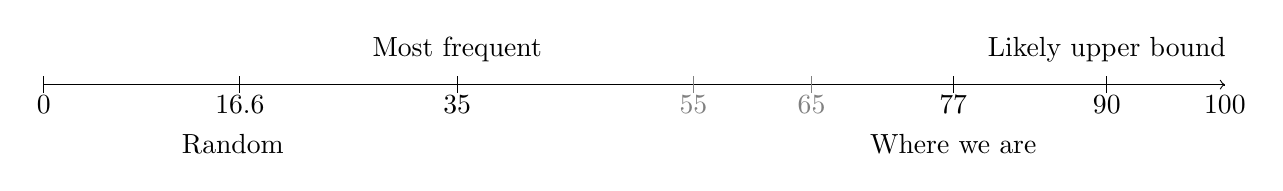
\begin{tikzpicture}[scale=0.15]
\draw[latex-latex,->] (0,0) -- (100,0) ; %edit here for the axis

\foreach \x in  {0,16.6,35,77,90} % edit here for the vertical lines
\draw[shift={(\x,0)},color=black] (0pt,20pt) -- (0pt,-20pt);

\draw[shift={(55,0)},color=gray] (0pt,20pt) -- (0pt,-20pt);
\draw[shift={(65,0)},color=gray] (0pt,20pt) -- (0pt,-20pt);

\foreach \x in {0,16.6,35,77,90,100} % edit here for the numbers
\draw[shift={(\x,0)},color=black] (0pt,0pt) -- (0pt,-3pt) node[below] {$\x$};

\draw[shift={(55,0)},color=gray] (0pt,0pt) -- (0pt,-3pt) node[below] {55};
\draw[shift={(65,0)},color=gray] (0pt,0pt) -- (0pt,-3pt) node[below] {65};
\node at (16,-5) {Random};
\node at (35,3) {Most frequent};
\node at (77,-5) {Where we are};
\node at (90,3) {Likely upper bound};
%\draw[*-o] (0.92,0) -- (2.08,0);
%\draw[very thick] (0.92,0) -- (1.92,0);
\end{tikzpicture}





\end{document}